\documentclass{article}
\usepackage{paper}

\setpapertitle{Interpretable Generative Models \\ for Molecule Design}

\tikzset{
	box/.style={
		rectangle,
		rounded corners,
		draw=black, very thick,
		minimum height=2em,
		inner sep=10pt,
		text centered,
	}
}

\begin{document}
\makeheader

\abstract{
	A recent advance in automatic molecular design is the use of generative latent variable models, particularly models based on the variational autoencoder framework. Such models, mostly based on Gaussian latent variables, offer excellect reconstruction and generative capabilities, however, afford little to no interpretability. I propose to resolve this issue by using binary latent variables. The proposed model is based on the state of the art architecture for molecular design, the Junction Tree VAE in which, similar to vanilla VAEs, the latent variables are gaussian and, therefore, offer no interpretability. Using binary latent variables fixes this situation and, coupled with an expressive Restricted Boltzmann Machine (RBM) prior, offer both interpretability and predictive powers of the original model. The learning is based on the Gumbolt approach which relies on smoothening the discrete latent space while gradient computation to facilitate backpropogation over the autoencoder network. I present a quantitative as well as qualitative analysis on the reconstruction and sampling on the ZINC dataset.
}

\begin{psection}{Introduction}

	The key challenge in automatic molecular design is to find molecules exhibiting similar behaviours to existing known molecules. The problem is challenging for two reasons: molecular design involves constructing coherent and feasible molecules; and we need to find continuous representations for molecules to find structurally similar molecules for efficient searching. Probabilisitic deep generative models, more particularly models based on Variational Autoencoders (VAEs), offer excellent frameworks to tackle the forementioned challenges. They allow learning and exploring molecular structure by decomposing the learning task to two complementary subtasks: learning to encode molecules in a smaller latent space that are representative of the molecule's structure; and learning to map an optimized representation back into a molecular structure.

	Amongst the two widely used deep generative models, Generative Adversarial Networks and VAEs, I limit my focus to VAE based models which aim to learn generative concept representations (or latent representations) using artificial neural networks comprising of the encoder. The second part consists of the decoder network which generates samples from the latent space and decodes them back to the feature spaces. Most VAE based models for molecular design modify the encoder and decoder networks to accomodate for generation and reconstruction of molecular structures.

	Specifically, these models start by generating a molecular representation of the molecule and translate them to a continuous latent representation (using gaussian latent variables) and reconstruct these latent representations using the decoder network. I start with providing a short background on the problem of molecular design and molecular representaions used in deep generative modelling. In Section 3, I present a brief survey on some of these models and discuss their limitations. In Section 4, I discuss in detail a state of the art method, Junction Tree VAE (JT-VAE), proposed by \cite{jtvae}, upon which the proposed approach is baed. Finally in Section 5 I discuss the changes made to the JT-VAE model to and a comparison of the results obtained by doing so. This is accompanied with a qualititative analysis of the modified JT-VAE model.

\end{psection}

\begin{psection}{Background on Molecular Design}

	Figure \ref{fig:mol-design} shows an abstract view of the major components which go into molecular design using generative models. 

	\begin{figure}[htpb]
		\centering
		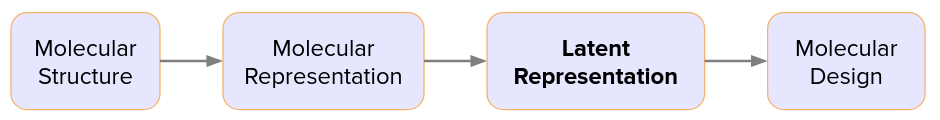
\includegraphics[width=\textwidth]{includes/mol-design.png}
		\caption{Steps to molecular design using generative models}
		\label{fig:mol-design}
	\end{figure}

	\begin{psubsection}{Molecular Representation}
		Although it is easy for us to understand the structure of a molecule by looking at its skeletal structure, they are inherently not machine understandable. Molecular representations provide machine-readable representations of these molecular structures. Molecular representations are therefore crucial to the design of a model since they dictate the generative capabilities of the model. There are multiple machine-readable molecular representations based on line notations or graph notations. A line notation named as Simplified Molecular-Input Line-Entry System (SMILES)  \citep{smiles} is widely used accross deep learning for it allows learning and generation using sequence based networks (such as Recurrent Neural Networks). Many recent models, however, are shifting towards graph based notations of molecular structure. The reason behind is the non-contuinity of SMILES representation across molecular structures. This is discussed in a bit more detail in the following text.

		\begin{pssubsection}{SMILES}

			SMILES \citep{smiles} is based on line notation of the molecular structure, \ie it deterministically transforms a molecular structure into a string based notation. The benefit of this, as pointed out earlier, is that these SMILES strings allow sequential learning and generation and, therefore, afford a wide set of models based on deep learning. SMILES can also used in a variety of ways: string, list of tokens, parse tree, or even as a molecular graph. Figure \ref{fig:smiles} shows an example of the SMILES representation of a skeletal structure of an organic molecule.

			\begin{figure}[htpb]
				\centering
				\raisebox{-0.5\height}{
					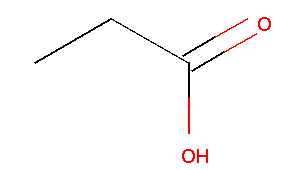
\includegraphics[height=80px]{includes/smiles-example.png}
				}
				\hspace{0cm}
				\raisebox{-0.5\height}{
					\resizebox{!}{40px}{
						\begin{tikzpicture}[->]
							\node at (-2.5, 0) {$\lra$};
							\node[box] {CCC(=O)O};
						\end{tikzpicture}
					}
				}
				\caption{An example of a SMILES string}
				\label{fig:smiles}
			\end{figure}

			Generative models use SMILES strings to compute latent representations and decode samples from the latent space back to SMILES strings. The problem with a naive approach, however, would be that the SMILES strings might not be syntactically and/or semantically coherent, or even if they are, they might not form reasonable molecular structures.

			Another problem with SMILES that makes optimizing on molecular properties in the latent space difficult is the discontinuity between two structurally similar molecules. This is demonstrated in Figure \ref{fig:smiles-problem}. To be precise, the SMILES strings of two structurally very similar molecules can be dissimilar, and therefore the latent representations in a generative model can be expected be be dissimilar as well. This is a cause for concern because the non-smooth latent space that is generated does not offer efficient searching for similar models for molecular design.

			\begin{figure}[htpb]
				\centering
				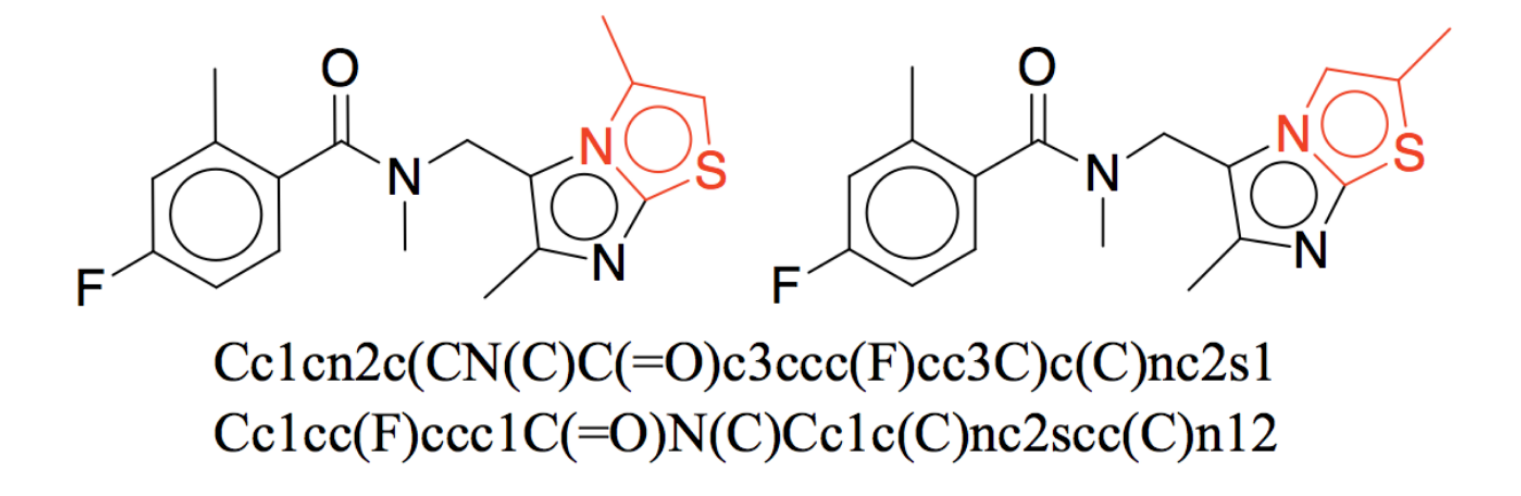
\includegraphics[width=0.8\textwidth]{includes/smiles-problem.png}
				\caption{Dissimilar SMILES string for structurally similar molecules}
				\label{fig:smiles-problem}
			\end{figure}

		\end{pssubsection}

		\begin{pssubsection}{Molecular Graph}

			A molecular graph encodes a molecular structure using a graph, where each atom is represented as a node and each bond is represented as an edge. Formally, a molecule M is represented as a graph $\sG = \para{\sV, \sE, \vu, \vv}$ where V and E represent the set of vertices and edges, respectively, and $\vu$ and $\vv$ are functions which assign features to each node and edge, respectively.

			Using molecular graphs for representing molecular structures in deep learning is benefitial as it allows us to apply graph convolutions, message passing algorithms, as well as sequential generation. This allows us to greatly advance our models for molecular design as is evident by recent models \cite{cgvae, jtvae}.

		\end{pssubsection}
	\end{psubsection}

\end{psection}

\begin{psection}{Molecular Design using Deep Generative Models}

	The general VAE architecture given in Figure \ref{fig:vae} is used to generate samples for molecular design. Recent models \citep{cvae, gvae, sd-vae, cgvae, jtvae} work upon this framework to encode different molecular representations to a continuous latent space using gaussian latent variables. As shown by these approaches, the latent space can be explored to find new molecular structures using optimization approaches \citep{jtvae} that afford superior properties to existing molecules.

	\begin{figure}[htpb]
		\centering
		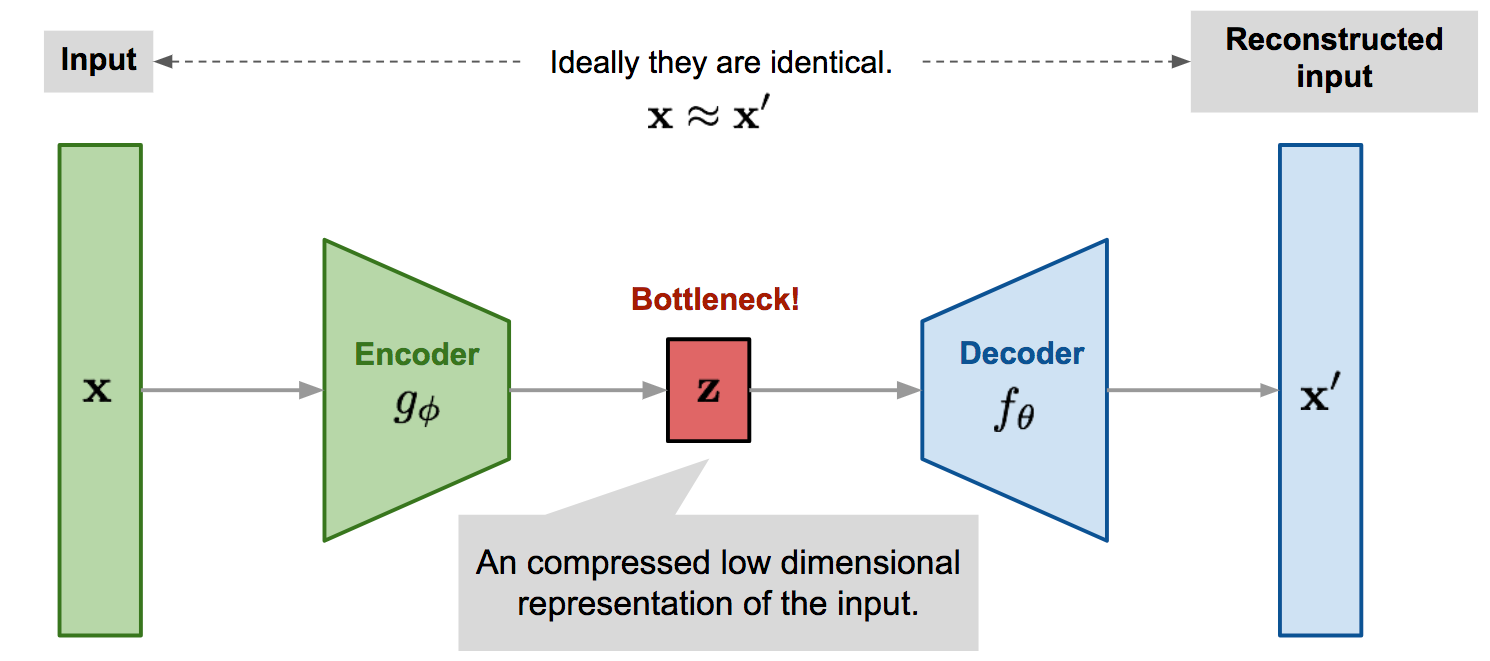
\includegraphics[width=0.8\textwidth]{includes/vae.png}
		\caption{Standard VAE architecture}
		\label{fig:vae}
	\end{figure}

	I discuss two categories of models: SMILES based models, and Molecular Graph based models and the developments and caveats each of them bring forth.

	\begin{psubsection}{SMILES based Deep Generative Models}

		\cite{cvae} introduced the first deep generative model for molecular design. Their approach is based on naive reconstruction and sampling of SMILES strings. Their goal was to learn a latent space wherein it is possible to interpolate, optimize and explore molecules with different properties. This is generously solved by using VAEs to encode the SMILES strings into continuous representations which allows effecient exploration. Their approach is straighforwardly based on minimizing the sum of the reconstruction loss and the kl-divergence of the gaussian variables with their standard normal priors, \ie the ELBO.

		\cite{cvae} modify the VAE architecture to encode and decode sequences using layered Gated Recurrent Units (GRUs) which allow for sequential encoding as well as sequential generation of the SMILES strings. In order to achieve latent representations that tend to predicting nice molecular properties, the ELBO is coupled with a property prediction loss to facilitate proper interpolation and exploration. 

		This approach, although being simple, faces the problem of having non-smooth latent space despite there being an addition classification loss acting as a regularizer. Moreover, due to sequential generation of the SMILES strings, the strings generated are often invalid (due to complex patters such as balanced paranthesis, etc.) and even if this is not the case, the SMILES strings do not correspond to reasonable models. Nonetheless, the continuous latent space allows for efficient Bayesian Optimization to guide the search for optimized molecular structures.

		\cite{gvae} present an alternate approach to generating molecular structures. Realizing the problems of using SMILES strings, Grammar Variational Autoencoder (GVAE) allows encoding and decoding parse trees. This allows us to generate SMILES parse trees rather than strings which fixes syntactic issues in the generated SMILES representations. Therefore, the latent space learnt is more coherent that that learnt by the previous model. The encoding and decoding are modeled in the same fashion as the naive approach.

		\cite{sd-vae} further extend the reconstruction of parse-tree from context-free grammars to attribute grammars which allows us to add semantics into the molecular representations. This approach allowed the generation of both syntactically and semantically valide SMILES. This, however, does not ensure that the molecule structures corresponding to these SMILES representations are feasible.

	\end{pssubsection}

\end{psubsection}

\begin{psubsection}{Molecular Graph based Models}

	The problem with SMILES, as highlighted earlier, is the discontuinity between molecular structures and molecular representations. An alternate strand of research focus on fixing this problem by utilizing molecular graph as the molecular representations. The earliest work on this approach by \cite{vaer} use Graph Convolution Networks (GCNs) to encode as well as decode the graphs. This allows reconstruction of the graphs while ensuring the continuous latent space to be coherent with the molecular structure, in contrast to models with SMILES based representations.

	Since it is possible that the reconstructed graphs are invalid and incongruent with the dynamics of molecular design, for example, disconnected graphs, or a six-carbon ring without aromatic bonds. \cite{vaer} attempt to fix this by adding penalties for such invalid generation, however, the model remains prone to such issues up to an extent.

	\cite{cgvae} builds upon the ideas of \cite{vaer} by updating the encoder and decoder networks to facilite sequential generation. They proposed Constrained Graph Variational Autoencoders (CGVAE) in which the latent representaion is obtained by encoding the molecular graph using message passing networks and is decoded using Gated Graph Neural Networks for alternating sequential generation of nodes and edges, accomponied by node and edge classification among valid candidates. Same as the model suggested by \cite{vaer}, CGVAE builds a continuous latent space congruent with the molecular structure and, therefore, offers efficient optimization, interpolation and exploration in the latent space.

	The problem, however, of generating unfeasible molecules still persists. Although the number of feasible samples generated using CGVAE are significantly higher than those generated using other aforementioned approaches, \cite{jtvae} propose a state-of-the-art model, Junction Tree VAE (JT-VAE), which obliterates this issue. The latent space mapped in JT-VAE is coherent with the molecular structure and the model generates only samples that are feasible. Moreover, JT-VAE even outperforms all previous models at the tast of reconstruction, whilst generating a smooth latent space optimal for exploration, optimization, etc.

\end{psubsection}

\end{psection}

\begin{psection}{Junction Tree Variational Autoencoders}

	Junction Tree Variational Autoencoder (JT-VAE) \citep{jtvae} is based on generating molecular graphs and does so, essentially, in two phases
	\begin{enumerate}
		\item It generates a tree-structured object (a junction tree) that  represents  the  scaffold  of subgraph  components and  their  coarse  relative  arrangements
		\item The subgraphs (nodes in the junction tree) are assembled into a coherent molecule graph using a graph message passing network. This approach incrementally generates the molecular graph while maintaining molecular validity at every step.
	\end{enumerate}

	Thus, the JT-VAE encoder has two parts: graph encoder and tree encoder, so has the decoder: tree decoder and graph decoder. The graph and tree encoders are closely related to message passing neural networks (MPNNs). The molecular structure, or rather the molecular graph, is encoded into a two-part continuous latent representation $\vz = \para{\vz_\sT, \vz_\sG}$ where $\vz_\sT$ encodes the tree structure and what the subgraph components are in the tree. $\vz_\sG$ encodes the graph to capture the fine-grained connectivity

	Both the molecular graph and junction tree are encoded via message passing using adapted gated recurrent units (GRUs). The junction tree is sequentially generated with message passing in a top-down as well as bottom-up (Contains topological and label predictions). Graph decoding, on the other hand, is performed in an alternating manner where a subgraph (for each node of the tree) is updated by evaluating a scoring function and making updates to maximize this scoring function (for details, refer to \citep{jtvae}).

	JT-VAE offers the most smooth latent space offering when compared to any of the earlier methods. Moreover, the samples generated using JT-VAE are all feasible. This is due to maintaining molecular validity at every step while generating the molecular graph from the junction tree and due to the fact that any junction tree that can be formed will give rise to at least one valid molecule.

	Although this model offers excellent optimization and exploration possibilities within the latent space, the one problem that can be identified is that the latent space, though smooth, remains non-interpretable. It is impossible to say what kind of molecule will be generated when samples are generated from a local neighbourhood. I attempt to remedy this by using binary variables along with gaussian latent variables to offer both interpretability of community structure and the expressiveness and smoothness of continuous latent variables.

\end{psection}

\begin{psection}{BBVI for Discrete Latent Variables: A Survey}

	\begin{psubsection}{Black Box Variational Inference}

		Black Box Variational Inference \citep{bbvi} is based on stochastic optimization of the variational objective. This allows us to perform model free analysis, which standard variational inference does not afford. Black box inference estimates the gradients of the variational objective (the ELBO) using Monte Carlo samples from the proxy posterior distribution. This can be derived by computing the gradients of the ELBO, which is written as below.
		\begin{align}
			\elbo{\vx, \vphi}	&\eq \E[\vz \sim q(\vz \spipe \vx, \vphi)]{\logp{p(\vx, \vz)} - \logp{q(\vz \pipe \vx, \vphi)}} \\
			\implies \nabla \elbo{\vx, \vphi} &\eq \E[\vz \sim q(\vz \spipe \vx, \vphi)]{\nabla_\vphi \logp{q(\vz \pipe \vx, \phi)} \para{\logp{p(\vx, \vz)} - \logp{q(\vz \pipe \vx, \vphi)}}} \label{eq:score-function}
		\end{align}

		BBVI can be applied on most posterior estimation problems, with very few restrictions, however, the gradient estimates computed using this have high variance, and therefore are often unsuitable to use in practical scenarios. The reparameterization trick allows estimation of the ELBO gradients using samples from a noise distribution with an apt (deterministic) transformation from the noise variable to the latent variable in question. Reparameterization trick reduces the variance by much, and is most desirable in many cases.

	\end{psubsection}

	\begin{psubsection}{Reparameterization for BBVI}

		The formulation written in equation \ref{eq:score-function} is known as the Score Function method. In order to reparameterize, the latent variable is written as a deterministic transformation of a noise variable (say $\vepsilon$) using a function $f$ such that $\vz = f(\vepsilon)$. Equation \ref{eq:score-function} can then be written alternately as
		\begin{align}
			\nabla \elbo{\vx, \vphi} \eq \E[\vepsilon]{\nabla_{\vphi} \logp{q(f(\vepsilon) \pipe \vx, \vphi)} \para{\logp{p(\vx, f(\vepsilon)) - \logp{q(f(\vepsilon) \pipe \vx, \vphi)}}}}
			\label{eq:rep-trick}
		\end{align}

		The biggest problem with the reparameterization trick is the limited number of distributions to which the trick can be applied successfully. Moreover, this often includes model specific changes and therefore undermines the Block Box property of BBVI.

		Moreover, any extension to include a wider set of priors to the reparameterization does not include the capability to handle discrete latent variables. In fact, it is not possible to use reparameterization with discrete latent variables because of the need to compute gradients over the latent variables which would be unbounded if the latent variable space is discrete.

	\end{psubsection}

	\begin{psubsection}{Discrete Latent Variables and BBVI}

		Although it is theoretically possible to learn models with discrete latent variables using the Score Function method, however, this naive approach gives estimates of the gradients which are impractically high variance. This variance can be reduced by adding control variates, which essentially translates to the \st{Reinforce} strategy (a technique popular in the Reinforcement Learning framework).

		Even with this reduced variance, we still face other difficulties. As \cite{dvae} points out, to capture an efficient estimate of the variance of a D-dimensional latent variable, we need at least D samples. Since a model can effectively have 100s of latent variables, the number of samples required to estimate the gradients is huge, and therefore inefficient. On the contrary, when using reparameterization, even a single sample can effectively estimate the direction of the gradients, and therefore work effeciently in training such models. Walking this line of ideas, there exist models \citep{gumbel, dvae, dvae-sharp, dvae-pp, gumbolt} which replace the discrete latent variables with some continuous relaxations and optimize a consistent objective.

	\end{psubsection}

	\begin{psubsection}{Gumbel-Softmax Trick}

		The Gumbel-Softmax Trick \citep{concrete, gumbel} affords a smooth relaxation for categorical variables, based on the Gumbel distribution and the Sofmax trick (and hence the name).

		The Gumbel-Max trick dictates that sampling from a categorical variable can be achieved using the following reparameterization: sample K uniform random variables $u_k \sim \cU(0, 1)$ and reparameterize the categorical random variable $z$ as
		\begin{align*}
			z \eq \argmax{k \in \brac{K}} \logp{\alpha_k} - \log{-\logp{u_k}}
		\end{align*}
		where $\alpha_k$ represents the unnormalized probabilty weight for class $k \in \brac{K}$.

		The variable $-\log{-\log{u_k}}$ is known to be from the Gumbel disitribution. This alternate sampling strategy allows us to write the relaxed version of the random variable $\vz$ (denoted by $\vz = \brac{z_1, z_2, \dots, z_K}$). which is then given as
		\begin{align*}
			z_k \eq \frac{\texp{\para{\logp{\alpha_k} + g_k} / \tau}}{\sum_{k' = 1}^K \texp{\para{\logp{\alpha_{k'}} + g_{k'}} / \tau}}
		\end{align*}
		where $\set{g_k}$ are i.i.d. samples from the gumbel distribution, and $\tau$ is a parameter, known as the temperature. It is obvious to see that as $\tau \ra 0$, the smooth relaxation $z_k \ra \is{z = k}$, and therefore as $\tau \ra 0$, $\vz$ would represent the one-hot form of $z$.

		In the ELBO term, the terms for the prior and posterior of the latent variable Z are replaced by simple relaxations to facilitate proper inference of the objective. This can be easily used to train binary latent variables, which is also shown in detail in \cite{concrete}. The problem, however, is that this relaxation is limited to simple categorical priors, and therefore does not scale to more complicated priors such as the Boltzman Machine prior.

	\end{psubsection}

	\begin{psubsection}{Restricted Boltzmann Machines}

		A boltzmann machine is an undirected probabilistic energy based model, where the probability mass for a binary (vector) latent variable, $\vz$, is given by
		\begin{align}
			\prob{\vz} \eq \frac{\texp{- E_\vtheta(\vz)}}{Z_\vtheta}
			\label{eq:bm-prob}
		\end{align}
		where $E_\vtheta(\vz)$ is the energy function, and $Z_\vtheta$ is the partition function, given by
		\begin{align*}
			Z_\vtheta \eq \sum_{\set{\vz}} \texp{- E_\vtheta(\vz)}
		\end{align*}

		Since the dimension of the variable $\vz$ can be large, it is impractical to compute the partition function, and therefore sampling needs to be used to estimate the value. In order to allow easier sampling (using Blocked Gibbs Sampling), we often assume the relation (undirected) between variables to be bipartite. This means that the set of variables $\vz$ is divided into two parts, $(\vz_1, \vz_2)$, and it is assumed that there is no link among the variables in $\vz_1$ and $\vz_2$ separately. This effectively means that given $\vz_1$, the probability of each variables in $\vz_2$ is independent, and vice versa. Such a model is known as the Restricted Boltzmann Machine (RBM). In the RBM literature, the variables $\vz$ are divided into visible and hidden variables, however since the models I discuss use RBMs as priors, we omit such distinction between the two sets of latent variables.

		The energy function in case of RBMs is given as
		\begin{align}
			E_\vtheta(\vz) \eq \va \cdot \vz_1 + \vb \cdot \vz_2 + \trans{\vz_2} \sW \vz_1
			\label{eq:energy-function}
		\end{align}
		where $\va$, $\vb$ and W are the biases (on $\vz_1$ and $\vz_2$ , respectively) and weights.

	\end{psubsection}

	\begin{psubsection}{GumBolt Trick}

		As pointed out earlier, the Gumbel Softmax trick is built for factorial distributions and does not scale to RBM priors. \cite{gumbolt} point out that the reason behind this is the removal of the latent variables $\vz$ from the inference model. Therefore, an alternate model, named as GumBolt is suggested by \cite{gumbolt} using the Gumbel-Softmax trick along with RBM priors.

		Similar to gumbel softmax case, a relaxed probabilities are required to replace the prior and the posterior probabilities. The posterior probability is consistent with the reparameterization offered by the Gumbel-Softmax Trick, however, the prior probability is replaced with a proxy, which is given as
		\begin{align}
			\widetilde{p}\para{\vzeta \pipe \vtheta} \eq \frac{\exp{-E_\vtheta(\vzeta)}}{Z_\vtheta}
			\label{eq:gumbolt-prob-proxy}
		\end{align}
		where $Z_\vtheta$ is the partition function for the prior probability of $\vz$. Note, the above proxy is not really a probability distribution, as it is unnormalized, however, as the temperature (of the Gumbel-Softmax trick) limits to 0, the above proxy tends to $\pp{\vz \pipe \vtheta}$. Moreover, the inconsistency of the posterior remaining a probability density function even when the temperature parameter limits to 0 is solved by replacing the posterior with a relaxed probability given as $\logp{\widetilde{q}\para{\vzeta \pipe \vx, \vphi}} = \vzeta \cdot \log{q} + (1 - \vzeta) \cdot \log{1 - q}$, where $q$ is the short-hand notation for $\qp{\vzeta \pipe \vx, \vphi}$. Therefore, the relaxed ELBO is written as
		\begin{align}
			\widetilde{\cL}(\vx, \vphi) \eq \E[\qp{\vzeta \spipe \vx, \vphi}]{\logp{\frac{\exp{-E_\vtheta(\vzeta)} \pp{\vx \pipe \vzeta, \vtheta}}{\widetilde{q}\para{\vzeta \pipe \vx, \vphi}}}} - \logp{Z_\vtheta}
			\label{eq:gumbolt-elbo}
		\end{align}

		As the temperature, $\tau \ra 0$, the $\widetilde{\cL}(\vx, \vphi) \ra \elbo{\vx, \vphi}$. The authors prove this ELBO to be a lower bound on the actual ELBO, and therefore claim that optimizing this ELBO with annealing temperature optimizes the actual object. This approach has another advantage over the Gumbel Softmax trick, this being that the Gumbolt proxy ELBO allows the use of importance weighted samples, which has shown to converge better than the standard ELBO, as it is an upper bound on the traditional ELBO. Use of RBM priors and Importance Weighted samples gives Gumbolt models an upperhand over the standard VAE with the Gumbel-Softmax Trick.

	\end{psubsection}
\end{psection}

\begin{psection}{Gumbolt Junction Tree Variational Autoencoder}

	In order to add interpretibility to the JT-VAE model, we ought to use discrete latent variables. Binary latent variables with a RBM prior seem to be fecilitous for this, however, experiments showed that the loss of expressiveness in the model due to binary variables had a largely negative effect on the reconstruction capabilities of the model. In order to fix this, I used continuous gaussian latent variables ($\vr \in \bR^{M}$) in company with the binary variables ($\vb \in \set{0, 1}^{M}$), and the final latent representation is given as an elementwise product of the two latent vectors, \ie $\vz = \vb \odot \vr$. We model the encoder and the decoders similar to JT-VAE, which are described as follows. Note that the latent space is still continuous despite introduction binary variables, and therefore it still offers the possibility of exploration and optimization.

	\begin{psubsection}{The VAE Decoder}

		The prior for the binary latent variables is given using an RBM prior. The variables are, therefore, decomposed into two sets, hidden and visible as $\vb = \brac{\vb_\sG, \vb_\sT}$ (therefore the partition is among variables for graph and tree respectively), and are then sampled from an RBM prior as follows
		\begin{align}
			\vb_\sG, \vb_\sT \qsim \text{RBM}(\va_\sG, \va_\sT, \sW)
			\label{eq:gvgcn-prior-binary}
		\end{align}
		The continuous variables are simply assumed to be sampled from a standard gaussian distribution as follows
		\begin{align}
			\vr \qsim \ND{\vzero, \vI}
			\label{eq:gvgcn-prior-binary}
		\end{align}
		The rest of the decoder network is the same as was used in JT-VAE, \ie based on an adapted message passing networks for sequentially generating trees followed by sequential generation of the graph from the predicted junction tree (for details, refer to \citep{jtvae}). The latent representation used $\vz$ is split into two parts as $\vz = \para{\vz_G, \vz_T}$ to be utilized for generating the final molecular graph.

		In order to avoid error propogation over incorrect predictions, teacher forcing is used as is common in sequence prediction.

	\end{psubsection}

	\begin{psubsection}{The VAE Encoder}

		The encoder network is the same as that used in JT-VAE with changes only in defining the posterior probabilities. Suppose we have the hidden representations $\vh_\sG$ and $\vh_\sT$ as outputs from the encoder network, which as mentioned earlier is a coupled variant of the MPNN. Therefore, we have $\set{\vh_\sG, \vh_\sT} = \tfunc{MPNN}{\vX, \sA}$ where $\vX$ represents the properties of all nodes and A represents the adjacency matrix holding information about the edge properties.

		The posterior is now given as a hierarchical posterior along with mean field assumption which assumes conditional independence of the binary variables given the hidden representations $\para{\vh_T, \vh_G}$ and assumes conditional independence of the gaussian variables given the hidden representations as well as the binary variables. Therefore, we can write the posterior as
		\begin{align}
			\func{q}{\vb, \vr \pipe \vX, \sA, \vphi} \eq \prod_{m = 1}^M \func{q}{b_m \pipe \vX, \sA, \vphi} \func{q}{r_m \pipe \vX, \sA, \vphi}
			\label{eq:posterior}
		\end{align}

		For consistency with the prior, we model the probabilities $\func{q}{b_m \pipe \vX, \sA}$ and $\func{q}{r_m \pipe \vb, \vX, \sA}$ using the bernoulli and the gaussian (respectively) distributions. The parameters for these distributions are computed by applying FC layers on the hidden representations obtained. We write this as
		\begin{align*}
			\func{q}{b_m \pipe \vh, \vphi} &\eq \text{Bernoulli}\para{\pi_m} \\
			\func{q}{r_m \pipe \vh \vphi} &\eq \ND{\mu_m, \sigma_m^2}
		\end{align*}
		where $\vh = \para{\vh_G, \vh_T}$, $\set{\pi_m}_{m = 1}^M = \tfunc{FC}{\vh}$, and $\set{\mu_m, \sigma_m}_{m = 1}^M = \text{GCN}(\vh, \vb)$.

		In order to infer the parameters, stochastic gradient variational bayes (SGVB) is used. Since this does not support binary (rather, discrete) latent variables, we use the Gumblt Probabilty proxy to compute the gradients of the KL term. The samples from the prior are generated using Persistive Contrastive Divergence. This allows us to efficiently train the model, while affording the greater expressive power of RBM priors in a generative setting. The reconstruction loss terms are modeled in the same way as is done in JT-VAE.

	\end{psubsection}

\end{psection}

\begin{psection}{Results}

	Tables \ref{tab:recon} and \ref{tab:accs} shows a comparison between JT-VAE and Gumbolt JT-VAE on different fronts. The topological, classification and assembly accuracies pertain to different tasks performed while decoding with teacher forcing. The observations tell us that the expressive power of Gumbolt JT-VAE is increased with the lower reconstruction loss and higher observed accuracies.
	\begin{table}[htpb]
		\centering
		\begin{tabular}{|c|c|}
			\hline
			\bt{Gumbolt JT-VAE} & \bt{JT-VAE} \\
			\hline
			3.889 & 4.019 \\
			\hline
		\end{tabular}
		\caption{Reconstruction Loss}
		\label{tab:recon}
	\end{table}

	\begin{table}[htpb]
		\centering
		\begin{tabular}{|l|c|c|}
			\hline
			& \bt{Gumbolt JT-VAE} & \bt{JT-VAE} \\
			\hline
			\bt{Topological Accuracy} & 93.38 & \bt{94.16} \\
			\hline
			\bt{Classification Accuracy} & \bt{99.21} & 97.57 \\
			\hline
			\bt{Assembly Accuracy} & \bt{95.34} & 94.31 \\
			\hline
		\end{tabular}
		\caption{Model Accuracies}
		\label{tab:accs}
	\end{table}

	Figure \ref{fig:local} shows molecules generated within the same neighbourhood. In this case, the binary latent variables are kept constant while the gaussian variables are varied over the x and y axes. The molecules show that there is definite neighbourhood continuity and hence the latent space offers good localization and chance of interpolation, optimization and exploration.
	\begin{figure}[htpb]
		\centering
		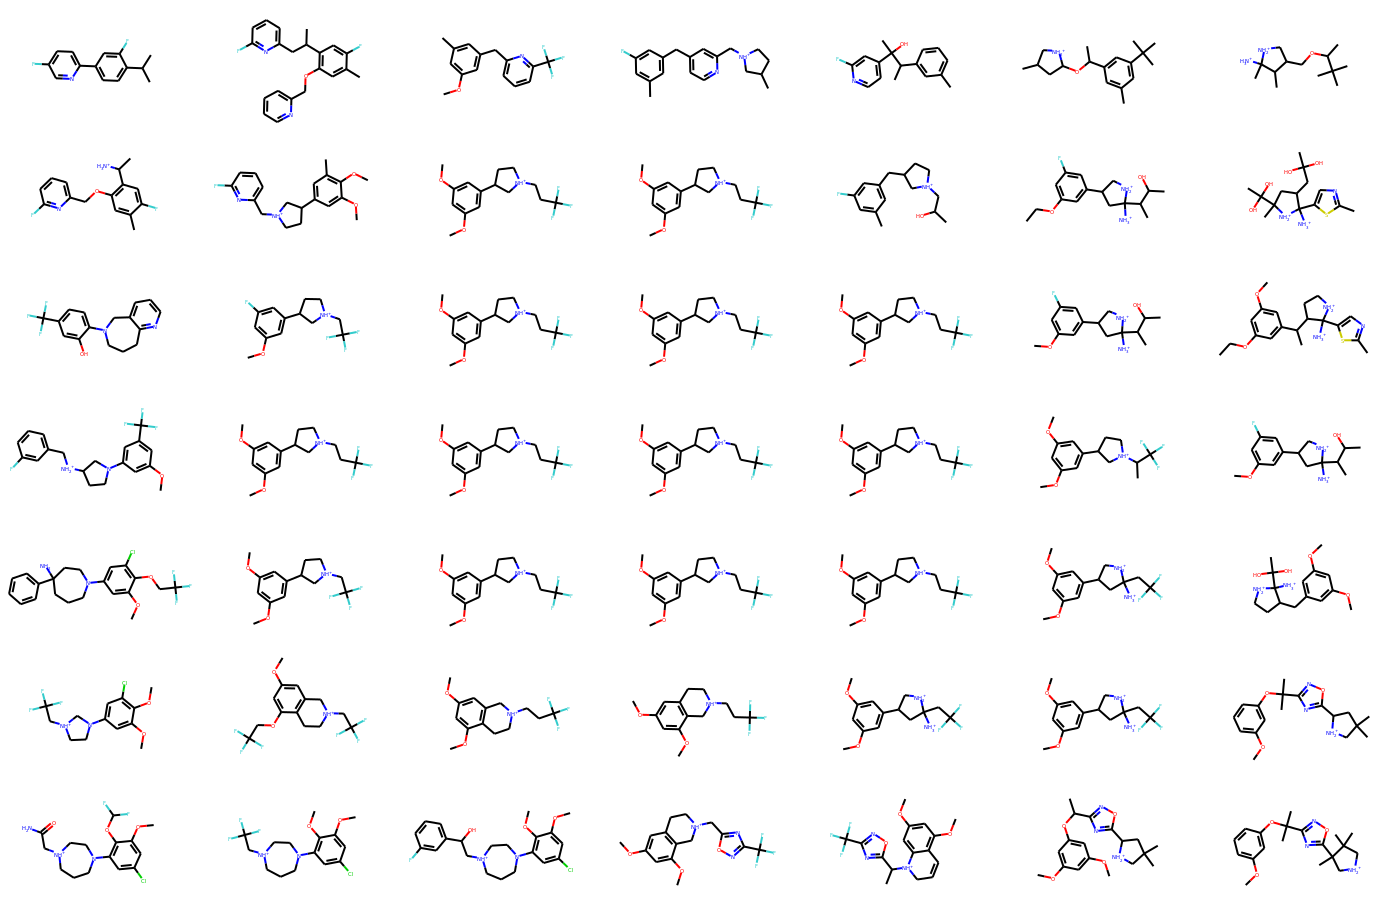
\includegraphics[width=\textwidth]{includes/plots/linear-local-samples.png}
		\caption{Generated samples from a local neighbourhood}
		\label{fig:local}
	\end{figure}

	In Figure \ref{fig:samples}, each column corresponds to the same binary latent variable and each row corresponds to the same gaussian variable. This figure shows the formation of communities up to some extend, however also has similarities accross rows. This analysis suggests that the efficacy of communities is therefore subdued. My belief is that this is occuring because of the contrained prior over the gaussian latent variables. Since we require the gaussian variables to be near 0, most of the values are too small. Because of this, even if change the values (similar to flipping bits) of some of the binary variables, there is minimal effect on the decoded structures.
	\begin{figure}[htpb]
		\centering
		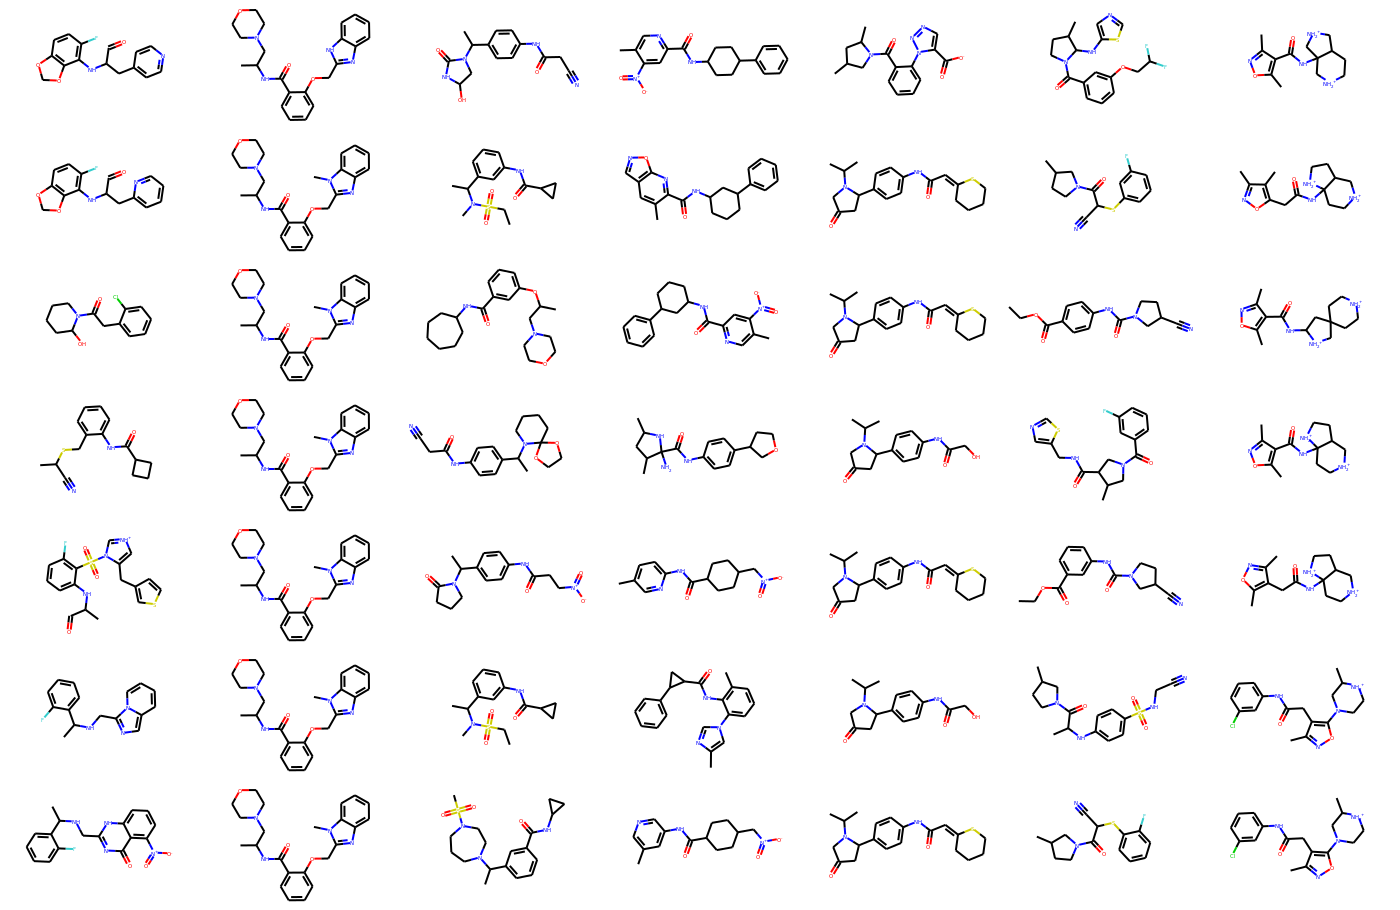
\includegraphics[width=\textwidth]{includes/plots/plots.png}
		\caption{Decoded molecules sampled from the prior}
		\label{fig:samples}
	\end{figure}

\end{psection}

\begin{psection}{Conclusion}

	I, in this project, have explored certain deep generative models for automatic molecule design. Most of the models offer contunous latent space yet lack the interpretability we would wish for in a sensitive task such as molecule design. In order to resolve this, I proposed to replace the gaussian variables with a set of binary variables accompanied by a set of gaussian variables depending upon the binary variables in the posterior. This allows us to have interpretability of binary variables while not losing any expressiveness.

	It is further possible to extend the model by replacing the KL-loss by Importance Weighted loss thereby ensuring faster convergence. Further, we could experiment by replacing teacher forcing with scheduled sampling. We can further improve upon the model by loosening the stringent and constraining prior requirements of the gaussian variables. I leave the task of exploring these directions for future work.

\end{psection}

\bibliographystyle{plainnat}
\bibliography{report}

\end{document}

